%source mathadata
%Objectif : tracer la droite séparatrice et comparer qualitativement les coefficients directeurs (signe, ...)
	Voici quatre graphiques représentant deux nuages de points~: les points verts et les points bleus. On cherche des équations de droites de la forme $y = mx + p$ qui séparent les nuages de points. Deux droites sont déjà tracées dans le graphique A et le graphique B.

	\begin{center}
		\begin{figure}[H]
			\centering
			\begin{subfigure}[t]{0.49\textwidth}
				\centering
				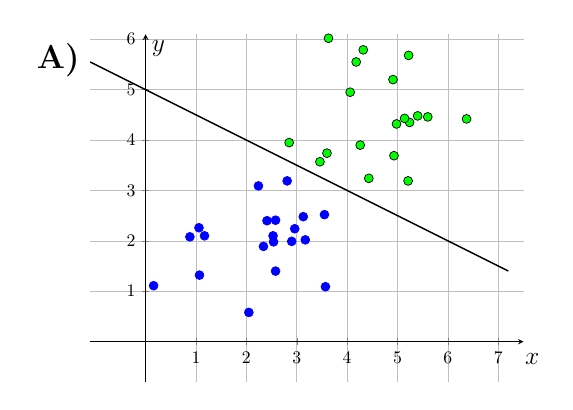
\begin{tikzpicture}[scale=0.64]
					\begin{axis}[
							name=plotA,
							x=1cm,y=1cm,
							axis lines=middle,
							ymajorgrids=true,
							xmajorgrids=true,
							xmin=-1.1,
							xmax=7.5,
							ymin=-0.8,
							ymax=6.1,
							xtick={1,...,7},
							ytick={0,1,...,6},
							xlabel={\Large $x$},
							xlabel style={at={(axis description cs:1.02,0.1)}, anchor=north},
							ylabel={\Large $y$},
							scatter/classes={
									A={mark=*,mark size = 2.5pt,draw=blue, fill = blue},
									B={mark=*,mark size = 2.5pt,draw=black, fill = green}
								}
						]
						\addplot[scatter,only marks,scatter src=explicit symbolic]
						coordinates {

								(2.53,2.1)[A]
								(2.05,0.58)[A]
								(2.41,2.4)[A]
								(3.55,2.52)[A]
								(2.24,3.09)[A]
								(1.07,1.32)[A]
								(2.58,1.4)[A]
								(0.88,2.08)[A]
								(2.81,3.19)[A]
								(1.06,2.26)[A]
								(3.17,2.02)[A]
								(3.13,2.48)[A]
								(1.17,2.1)[A]
								(2.96,2.24)[A]
								(2.54,1.98)[A]
								(2.9,1.99)[A]
								(0.16,1.11)[A]
								(2.58,2.41)[A]
								(3.57,1.09)[A]
								(2.34,1.89)[A]
								(5.3,7.37)[B]
								(6.37,4.42)[B]
								(4.18,5.55)[B]
								(4.26,3.9)[B]
								(5.22,5.68)[B]
								(4.91,5.2)[B]
								(4.43,3.24)[B]
								(2.85,3.95)[B]
								(4.98,4.32)[B]
								(5.4,4.48)[B]
								(4.93,3.69)[B]
								(5.24,4.35)[B]
								(4.32,5.79)[B]
								(3.63,6.02)[B]
								(3.6,3.74)[B]
								(5.6,4.46)[B]
								(5.14,4.43)[B]
								(5.21,3.19)[B]
								(4.06,4.95)[B]
								(3.46,3.57)[B]
							};
						% Line through (2,4) and (4,3) -> y = -0.5 x + 5
						\addplot[domain=-1.1:7.2, samples=2, thick] {-0.5*x + 5};

					\end{axis}

					% letter A) in top-left of axis
					\node[anchor=north west,font=\large\bfseries,xshift=-8mm] at (plotA.north west) {A)};
				\end{tikzpicture}
				%\caption{}
			\end{subfigure}
			\hfill
			\begin{subfigure}[t]{0.49\textwidth}
				\centering

				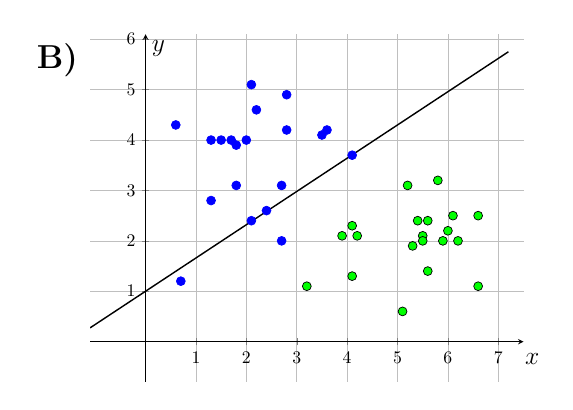
\begin{tikzpicture}[scale=0.64]
					\begin{axis}[
							name=plotB,
							x=1cm,y=1cm,
							axis lines=middle,
							ymajorgrids=true,
							xmajorgrids=true,
							xmin=-1.1,
							xmax=7.5,
							ymin=-0.8,
							ymax=6.1,
							xtick={1,...,7},
							ytick={0,1,...,6},
							xlabel={\Large $x$},
							xlabel style={at={(axis description cs:1.02,0.1)}, anchor=north},
							ylabel={\Large $y$},
							scatter/classes={
									A={mark=*,mark size = 2.5pt,draw=blue, fill = blue},
									B={mark=*,mark size = 2.5pt,draw=black, fill = green}
								}
						]
						\addplot[scatter,only marks,scatter src=explicit symbolic]
						coordinates {

								(0.7,1.2)[A]
								(0.6,4.3)[A]
								(2.4,2.6)[A]
								(2.8,4.2)[A]
								(1.3,2.8)[A]
								(1.8,3.1)[A]
								(2.8,4.9)[A]
								(4.1,3.7)[A]
								(2.0,4.0)[A]
								(1.5,4.0)[A]
								(2.2,4.6)[A]
								(1.7,4.0)[A]
								(2.1,2.4)[A]
								(2.7,2.0)[A]
								(3.5,4.1)[A]
								(1.3,4.0)[A]
								(1.8,3.9)[A]
								(2.1,5.1)[A]
								(2.7,3.1)[A]
								(3.6,4.2)[A]
								(5.5,2.1)[B]
								(5.1,0.6)[B]
								(5.4,2.4)[B]
								(6.6,2.5)[B]
								(5.2,3.1)[B]
								(4.1,1.3)[B]
								(5.6,1.4)[B]
								(3.9,2.1)[B]
								(5.8,3.2)[B]
								(4.1,2.3)[B]
								(6.2,2.0)[B]
								(6.1,2.5)[B]
								(4.2,2.1)[B]
								(6.0,2.2)[B]
								(5.5,2.0)[B]
								(5.9,2.0)[B]
								(3.2,1.1)[B]
								(5.6,2.4)[B]
								(6.6,1.1)[B]
								(5.3,1.9)[B]
							};

						% Line through (1,0) and (3,2) -> y = 0.66 x + 1
						\addplot[domain=-1.1:7.2, samples=2, thick] {0.66*x + 1};

					\end{axis}

					% letter B) in top-left of axis
					\node[anchor=north west,font=\large\bfseries,xshift=-8mm] at (plotB.north west) {B)};
				\end{tikzpicture}
				%\caption{}
			\end{subfigure}
			%\caption{}

			\vspace*{8pt}

			\begin{subfigure}[t]{0.49\textwidth}
				\centering
				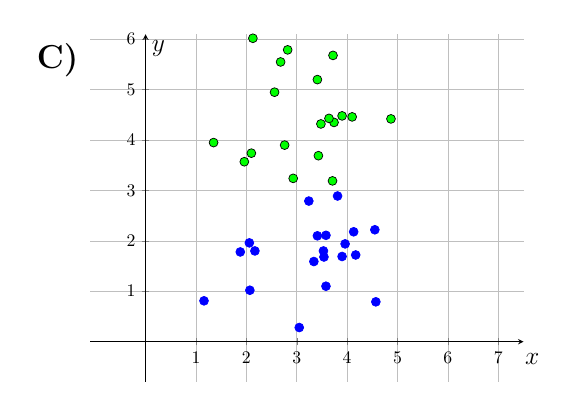
\begin{tikzpicture}[scale=0.64]
					\begin{axis}[
							name=plotC,
							x=1cm,y=1cm,
							axis lines=middle,
							ymajorgrids=true,
							xmajorgrids=true,
							xmin=-1.1,
							xmax=7.5,
							ymin=-0.8,
							ymax=6.1,
							xtick={1,...,7},
							ytick={0,1,...,6},
							xlabel={\Large $x$},
							xlabel style={at={(axis description cs:1.02,0.1)}, anchor=north},
							ylabel={\Large $y$},
							scatter/classes={
									A={mark=*,mark size = 2.5pt,draw=blue, fill = blue},
									B={mark=*,mark size = 2.5pt,draw=black, fill = green}
								}
						]
						\addplot[scatter,only marks,scatter src=explicit symbolic]
						coordinates {
								(3.53,1.8)[A]
								(3.05,0.28)[A]
								(3.41,2.1)[A]
								(4.55,2.22)[A]
								(3.24,2.79)[A]
								(2.07,1.02)[A]
								(3.58,1.1)[A]
								(1.88,1.78)[A]
								(3.81,2.89)[A]
								(2.06,1.96)[A]
								(4.17,1.72)[A]
								(4.13,2.18)[A]
								(2.17,1.8)[A]
								(3.96,1.94)[A]
								(3.54,1.68)[A]
								(3.9,1.69)[A]
								(1.16,0.81)[A]
								(3.58,2.11)[A]
								(4.57,0.79)[A]
								(3.34,1.59)[A]
								(3.8,7.37)[B]
								(4.87,4.42)[B]
								(2.68,5.55)[B]
								(2.76,3.9)[B]
								(3.72,5.68)[B]
								(3.41,5.2)[B]
								(2.93,3.24)[B]
								(1.35,3.95)[B]
								(3.48,4.32)[B]
								(3.9,4.48)[B]
								(3.43,3.69)[B]
								(3.74,4.35)[B]
								(2.82,5.79)[B]
								(2.13,6.02)[B]
								(2.1,3.74)[B]
								(4.1,4.46)[B]
								(3.64,4.43)[B]
								(3.71,3.19)[B]
								(2.56,4.95)[B]
								(1.96,3.57)[B]
							};
					\end{axis}

					% letter C) in top-left of axis
					\node[anchor=north west,font=\large\bfseries,xshift=-8mm] at (plotC.north west) {C)};
				\end{tikzpicture}
				%\caption{}
			\end{subfigure}
			\hfill
			\begin{subfigure}[t]{0.49\textwidth}
				\centering
				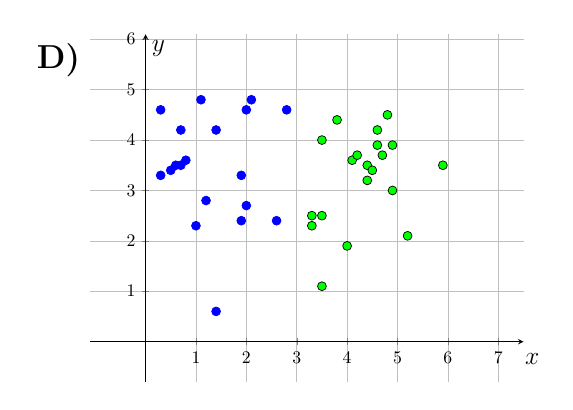
\begin{tikzpicture}[scale=0.64]
					\begin{axis}[
							name=plotD,
							x=1cm,y=1cm,
							axis lines=middle,
							ymajorgrids=true,
							xmajorgrids=true,
							xmin=-1.1,
							xmax=7.5,
							ymin=-0.8,
							ymax=6.1,
							xtick={1,...,7},
							ytick={0,1,...,6},
							xlabel={\Large $x$},
							xlabel style={at={(axis description cs:1.02,0.1)}, anchor=north},
							ylabel={\Large $y$},
							scatter/classes={
									A={mark=*,mark size = 2.5pt,draw=blue, fill = blue},
									B={mark=*,mark size = 2.5pt,draw=black, fill = green}
								}
						]
						\addplot[scatter,only marks,scatter src=explicit symbolic]
						coordinates {
								(1.4,0.6)[A]
								(2.0,2.7)[A]
								(1.4,4.2)[A]
								(1.0,2.3)[A]
								(1.2,2.8)[A]
								(1.1,4.8)[A]
								(2.8,4.6)[A]
								(0.8,3.6)[A]
								(0.5,3.4)[A]
								(0.7,4.2)[A]
								(0.6,3.5)[A]
								(1.9,2.4)[A]
								(2.6,2.4)[A]
								(2.0,4.6)[A]
								(0.3,3.3)[A]
								(0.7,3.5)[A]
								(0.3,4.6)[A]
								(1.9,3.3)[A]
								(2.1,4.8)[A]
								(4.4,3.5)[B]
								(5.2,2.1)[B]
								(4.1,3.6)[B]
								(4.8,4.5)[B]
								(3.5,4.0)[B]
								(4.0,1.9)[B]
								(4.9,3.0)[B]
								(3.3,2.3)[B]
								(3.8,4.4)[B]
								(3.3,2.5)[B]
								(4.9,3.9)[B]
								(4.6,4.2)[B]
								(3.5,2.5)[B]
								(4.6,3.9)[B]
								(4.5,3.4)[B]
								(4.7,3.7)[B]
								(3.5,1.1)[B]
								(4.2,3.7)[B]
								(5.9,3.5)[B]
								(4.4,3.2)[B]
							};
					\end{axis}

					% letter D) in top-left of axis
					\node[anchor=north west,font=\large\bfseries,xshift=-8mm] at (plotD.north west) {D)};
				\end{tikzpicture}
			\end{subfigure}
		\end{figure}
	\end{center}

	\vspace{-1cm}
	\begin{multicols}{2}

		\begin{MADenumerate}
			\item \textbf{Pour le graphique A :}
			\begin{enumerate}
				\item Quel est le signe du coefficient directeur $m$ ? Justifier graphiquement.
				\item Déterminer graphiquement la valeur $p$ de l'ordonnée à l'origine.
				\item Calculer le coefficient directeur $m$. (Utiliser la formule du taux d'accroissement pour deux points de la droite.)
				\item Écrire l'équation complète de la droite\\ $y=m x + p$ .
			\end{enumerate}

			\columnbreak

			\item \textbf{Pour le graphique B :}
			\begin{enumerate}
				\item Répondre aux mêmes questions que pour le graphique A.
				\item (Bonus) Proposer une autre droite qui sépare mieux les nuages de points et donner son équation.
			\end{enumerate}

			\item \textbf{Pour les graphiques C et D}, tracer une droite horizontale ou verticale qui sépare les nuages de points, puis écrire son équation.

		\end{MADenumerate}

	\end{multicols}
